\chapter{Fundamentação Teórica}

\section{Introdução}

Escrever Introdução

\section{Redes Neurais}
\label{sec:ewheelchair}

As redes neurais artificiais são modelos computacionais inspirados no funcionamento do cérebro humano, compostos por neurônios interconectados que processam informações. Elas são amplamente utilizadas em diversas áreas, como reconhecimento de padrões, processamento de linguagem natural, visão computacional e muitas outras aplicações de aprendizado de máquina. Em (\citeyear{rumelhart1986learning}), descreve-se pioneiramente o algoritmo de retropropagação, fundamental para o treinamento de redes neurais profundas.

\begin{figure}[!h]
\center
\begin{minipage}{0.45\linewidth}
\center
\captionsetup{justification=centering,margin=0.5cm,font=small}
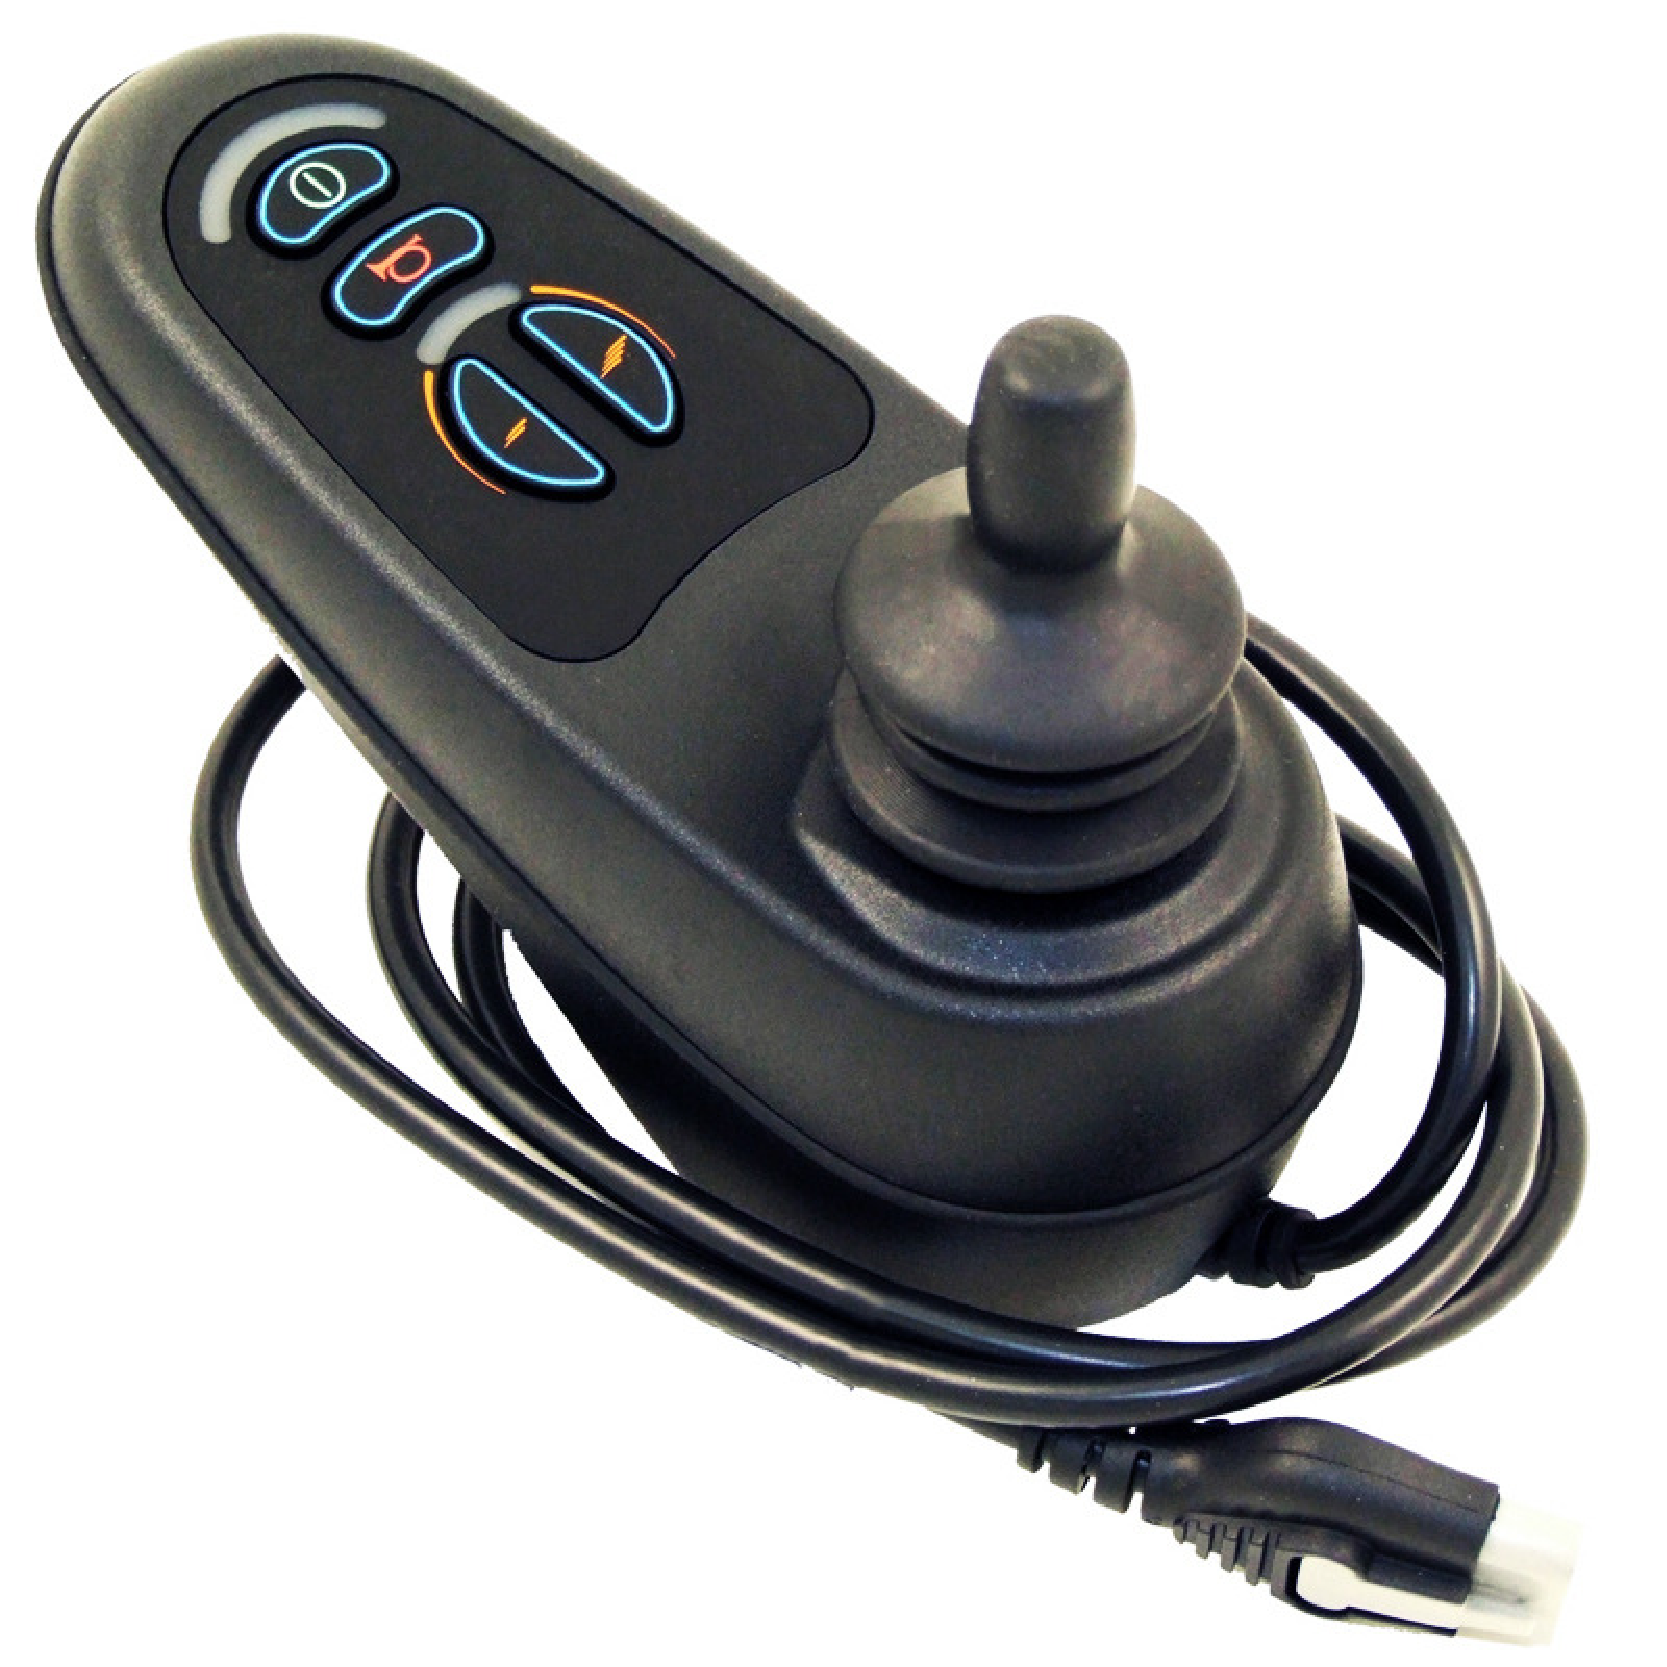
\includegraphics[width=0.7\linewidth]{img/cap2/joystickvr2}
\caption{ JoystickVR2 - JSM  \cite{joystickvr2jsm}} \label{subfig:joystickvr2}
\end{minipage}
\begin{minipage}{0.45\linewidth}
\center
\captionsetup{justification=centering,margin=0cm,font=small}
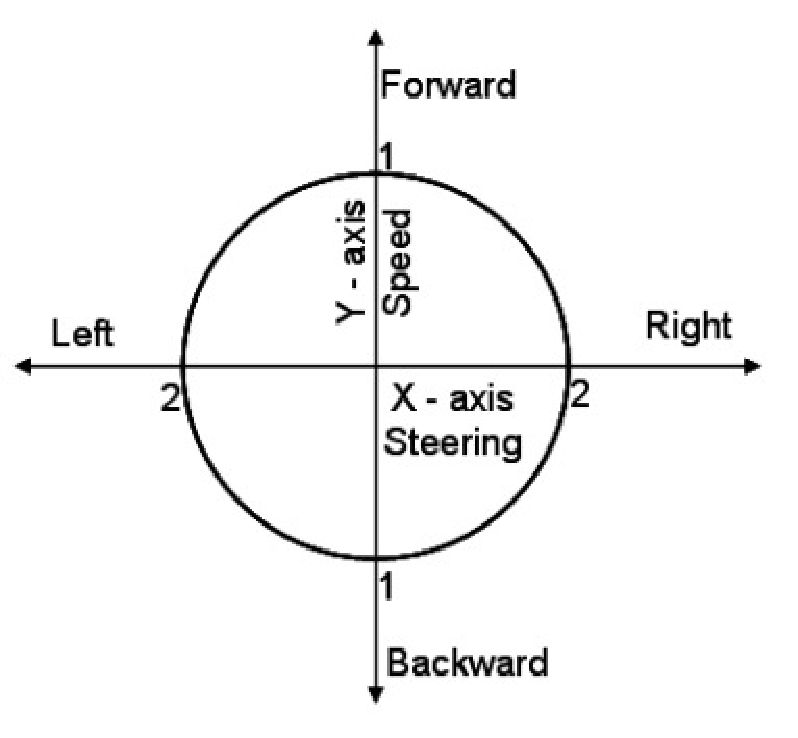
\includegraphics[width=0.8\linewidth]{img/cap2/joyscoord}
\caption{ Joystick axis interpretation \cite{fattouh2004}} \label{subfig:joyscoord}
\end{minipage}
\end{figure}

A joystick control interface cannot fully meet the needs of the disabled and elderly person whose autonomies are seriously affected by a decline in their motor function and cognitive performance \cite{rechy2012}. AT, like plug-in devices (Figures \ref{subfig:jck-ushape} and \ref{subfig:jck-ywlball}), have been developed over the years to facilitate joystick handling by users during the training sessions or in their Activities of Daily Living (ADL) and Instrumental Activities of Daily Life  (IADL)\cite{american2014, american2008}. 

However, there is a gap in Ordinance n. 1272 defined by the Unified Health System in Brazil that describes the mandatory training, monitoring and maintenance of use, maintaining the absence of systematized protocols and standardized norms and it might expose the users to further injuries \cite{valentini2019,portaria2013, anexos2013}. 

\begin{figure}[!h]
\center
\begin{minipage}{0.45\linewidth}
\center
\captionsetup{justification=centering,margin=0cm,font=small}
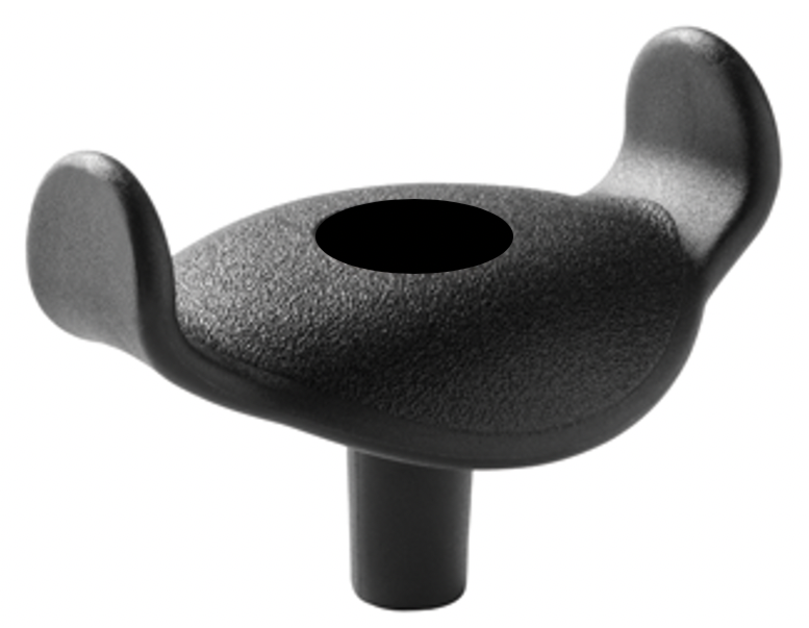
\includegraphics[width=0.85\linewidth]{img/cap2/jck-ushape}
\caption{ U-shaped joystick handle \cite{jck-ushape2020}} \label{subfig:jck-ushape}
\end{minipage}
\begin{minipage}{0.45\linewidth}
\center
\captionsetup{justification=centering,margin=0cm,font=small}
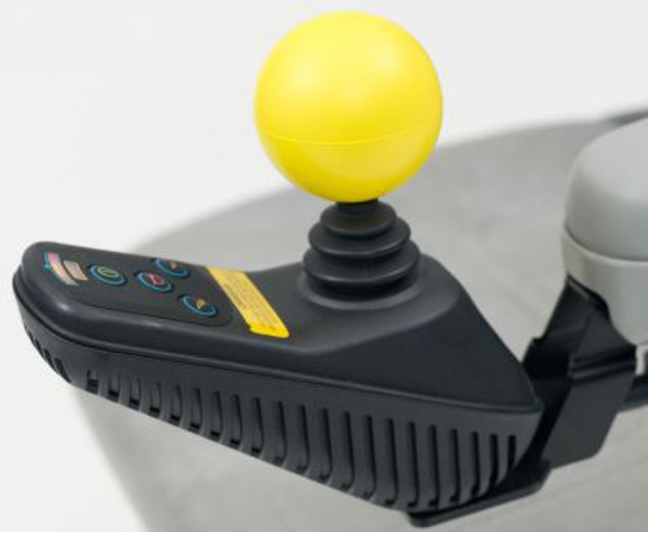
\includegraphics[width=0.8\linewidth]{img/cap2/jck-ywlball}
\caption{ Yellow joystick knob foam ball \cite{jck-ywlball2020}} \label{subfig:jck-ywlball}
\end{minipage}
\end{figure}

%Thus, the next section will present an introduction to these technologies.  

\section{Virtual and Augmented Reality}
\label{sec:vareality}

VR and AR have been used in different situations to provide safe conditions to the user's training or adaptation phase, with different devices and control interfaces. 

VR is an advanced user interface having, as main features, the ability for 3D visualization, spatial navigation and interaction in a 3D synthetic environment \cite{tori2006}. In many situations, access to a physical training environment can be restricted by some constraints such as time and space. The user still can not have a caregiver to take them to a therapist center or it may be expensive to move close by \cite{mitsumura2014}. When such limitations are faced, VR can be used to extend availability of training environments, also bringing the training exercises to the user. The use of technology to support rehabilitation is not a new phenomenon, improvements in hardware and cost reduction increased the interest in the use of VR \cite{wiederhold2019,powell2014}. 

Many researches in cognitive rehabilitation have been investigating the use of  VR techniques \cite{vailland2019,john2018, kamaraj2016, mahajan2013}. Among the main characteristics of these environments, there is the preservation of physical integrity of the user and training assessments. However, some users notice some difficult when using these systems. They face some limitations concerning the immersion that these environments offer.

AR optimizes the user experience since it creates an altered reality without losing the benefits of the physical setting \cite{wiederhold2019}. In the study conducted by Ines (2011), the use of AR techniques has proven to enhance user motivation and acceptance in many different situations \cite{ines2011}. 

For instance, in work presented by Manring et al. \cite{manring2020}, an augmented training environment was created using  Microsoft Hololens for controlling an interactive robot. Robots intervention is considered a high-risk task where practiced remotely by technicians or doctors. Robots are force-feedback devices that are not easy to operate, require high control accuracy, and also require extensive training by operators. For this reason, AR techniques were implemented to reduce the amount of training and increase the user skill to control the robot. Among the control, methods are: manual and automatic. The user can move the end effector of the holographic robot, and the physical robot will respond immediately, in manual control. Otherwise,  the user can move the end effector of the holographic robot to the desired location, view a holographic preview of the motion, and select execute if the motion plan is satisfactory, using automatic control. Figure \ref{fig:manring2020} illustrates  on \textit{left} side: ``The physical robotic arm has just moved to the position of the holographic arm'' and on \textit{right} side: ``Previewing motion operation''. It is possible to customize the AR rendering using fiducial AR markers or not. 

\begin{figure}[!hbt]
\begin{center}
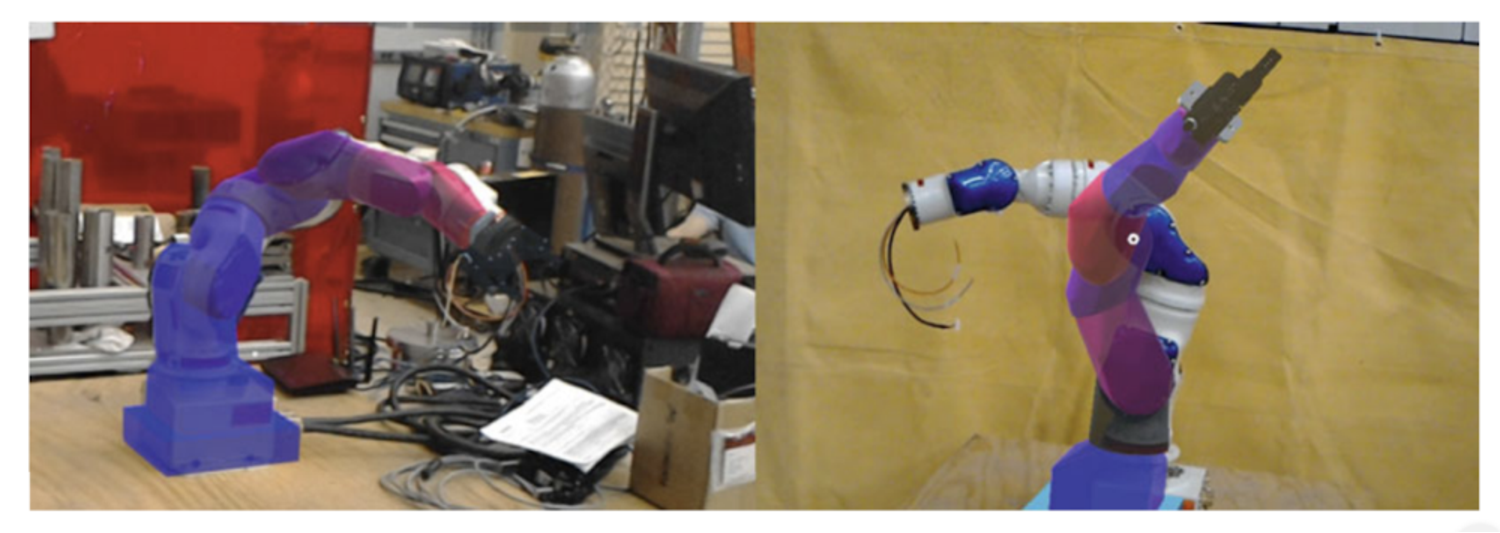
\includegraphics[width=1 \textwidth]{img/cap2/manring2020}
\caption{\textit{Left}: ``Automatic'' - \textit{Right}: ``Manual'' modes by \cite{manring2020}}
\label{fig:manring2020}
\end{center}
\end{figure}

Silva (2011) developed a distributed environment using AR techniques \cite{silva2011}. A shared AR environment is an exciting feature to be used in telerehabilitation situations. Thus, the user and therapist can interact at the same time with the environment making the user evolves more effectively. 


\section{PMRT training assessments}
\label{sec:trainingEvaluation}

In any rehabilitation/training process locally or remotely, to assess user performance is essential to be related to driver skills improvement \cite{macgillivray2018}. This evaluation process can be either carried out automatically or not \cite{john2018, massengale2005}. In the automatic method, a (statistical) calculation is performed based on the process metrics, without the intervention of the health professional\cite{john2018}. Or in non-automatic method, the health professional who holds the user's clinical information assigns a score, based on standard parameters \cite{massengale2005}.

Another important aspect in the evaluation process is to verify if it is performed in an interpersonal or intrapersonal way. The PMRT defined by Massengale et al. \cite{massengale2005} is a standard and reliable methodology (training and evaluation protocols) applied to each user (intrapersonal way) in a different way. The PMRT consists of 2 groups of tasks: structured and unstructured. The 12 structured tasks are predictable. The 4 unstructured / dynamic tasks are unpredictable and require the user to make decisions about interacting with the environment, such as avoiding a person walking down the corridor or avoiding a therapy ball on the way \cite{massengale2005}. The user is considered approved in a training protocol when he/she reaches a score higher than or equal to 95\%. All tasks assessed in the PMRT are based on visual perception of the professional in charge. Before attribute a task score, the health professional has to be aware of the following rules:
\begin{itemize}
\item 4 -  Completely independent: optimal performance: able to perform task in one attempt smoothly and safely;
\item 3 - Completes task hesitantly, requires several tries, requires speed restriction, and/or bumps wall, objects, etc. lightly (without causing harm);
\item 2 - Bumps objects and people in a way that causes harm or could cause harm to driver, other persons or to objects;
\item 1 - Unable to complete task: reason:  For example, may require verbal and/or visual cues or physical assistance.
\end{itemize} 

\section{Telerehabilitation}
\label{sec:telerehabilitation}

As defined in \cite{deutsch2007}, ``telerehabilitation is the provision of rehabilitation services (evaluations and interventions) at a distance by therapists at a remote location''. Over recent years, telerehabilitation technology has been developed seeking to address some issues related to classical in-clinic treatment \cite{pani2014,postolache2011}. Among these issues, one can highlight the one presented in Figure \ref{fig:holden2007}, which is the availability of the physical environment (and equipment) and the time and expenses associated to users and therapists displacement \cite{brennan2011,holden2007,dhurjaty2004}.

\begin{figure}[!hbt]
\begin{center}
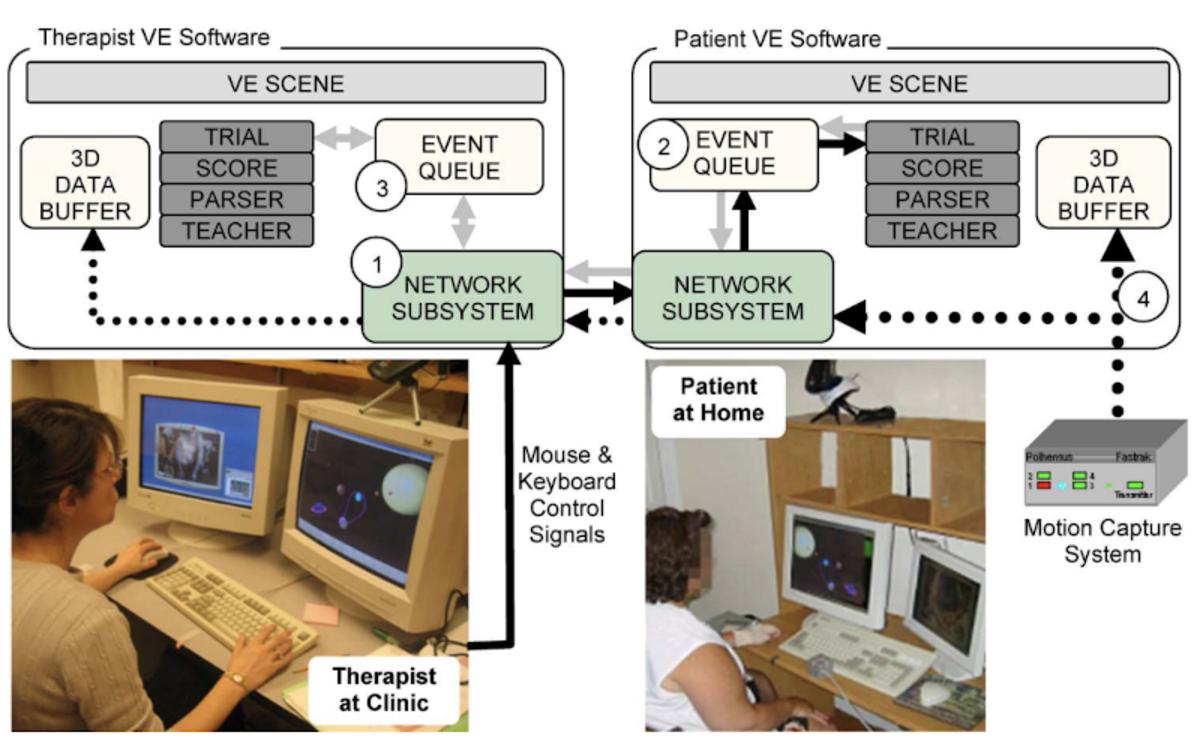
\includegraphics[width=1 \textwidth]{img/cap2/holden2007}
\caption{Virtual telerehabilitation system \cite{holden2007}}
\label{fig:holden2007}
\end{center}
\end{figure}

Telerehabilitation technology can be used to improve existing rehabilitation protocols. Since many standard treatments include a high number of repetitive exercises, users are required to perform additional exercises at home, without the supervision of a therapist \cite{ortiz2014}. In these cases, telerehabilitation software can be used to provide the therapist with valuable feedback. As stated by \cite{ortiz2014}, ``the monitoring of quality and quantity of home-based rehabilitation interventions can potentially have a large positive impact on the quality and adherence to long-term treatments and rehabilitation outcomes'' \cite{pons2014}. Finally, it is important to mention that telerehabilitation applications run over pure network (UDP or HTTP -- Hypertext Transfer Protocol) protocol sockets \cite{leung2007}.

\section{Web server applications}
\label{sec:websapp}

Currently, with the intensive use of Internet, fast development of web technologies and high-performance computer hardware, building web sites and constructing software systems on the web are dominant trends in the e-commerce industry \cite{attitalla2016, zambonelli2016,laine2011,stroulia2001}. 

Web server-based approaches allow controlling devices and appliances remotely. Two methods are being used: one is to develop an embedded web server using dedicated hardware, and  the other is to use Cloud-based services and develop the application on it, without the need for hardware, latency or network failure \cite{attitalla2016}. 

Researchers \cite{tilley2001}  classify web sites architectures in three categories, according to their level of complexity, interactivity and functionality:
\begin{itemize}
\item Static: plain HyperText Markup Language (HTML) web sites;
\item Interactive (Front-end side): dynamic HTML plus some scripting programs (e.g., JavaScript); and
\item Dynamic (back-end site): powerful server-side systems that can generate web contents dynamically.
\end{itemize}

\begin{figure}[!h]
\center
\begin{minipage}{0.45\linewidth}
\center
\captionsetup{justification=centering,margin=0cm,font= small}
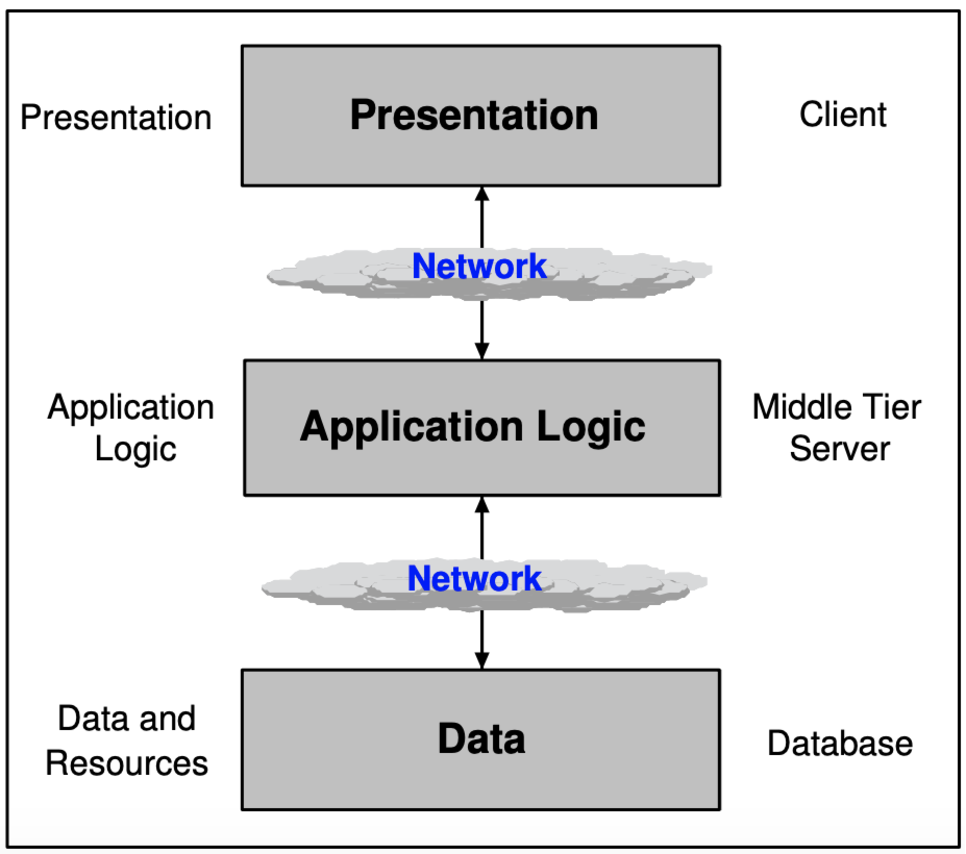
\includegraphics[width=0.85\linewidth]{img/cap2/webTierarch}
\caption{ A typical three-tire architecture \cite{sun2003} } \label{subfig:webTierarch}
\end{minipage}
\begin{minipage}{0.45\linewidth}
\center
\captionsetup{justification=centering,margin=0cm,font= small}
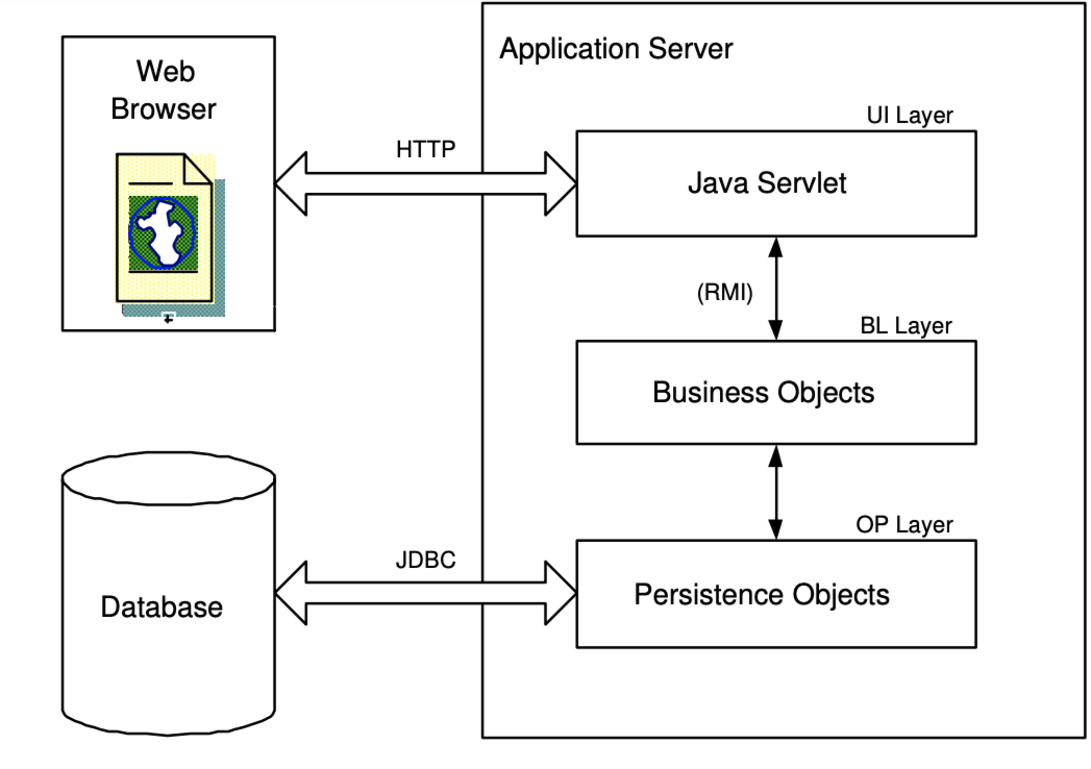
\includegraphics[width=1.05\linewidth]{img/cap2/firstWebArch}
\caption{ The first version architecture \cite{sun2003}} \label{subfig:firstWebArch}
\end{minipage}
\end{figure}

The dynamic web application architectures presented in Figures \ref{subfig:webTierarch} and \ref{subfig:firstWebArch} allows one to:

\begin{itemize}
\item Manage image/videos streams in order to provide a powerful visual feedback from user;
\item Establish different channels to receive/redirect all different kinds of data coming from different user control interfaces;
\item Save all data generated during user experience allowing for the processing of this data creating indicator measurements across the acquired evolution and;
\item Operating system and platform independence, as long as it is supported in the
browser.
\end{itemize}

Throughout the web server features, it's possible to develop a cross platform application which can be accessed for everyone from different places in the world. Different modules can be implemented based in Java Servlets. Each kind of data from different devices all over Internet, can be handled for different modules. For instance, video stream manager to visualize different physical places,   store different real time data to generate reports \cite{attitalla2016, kovatsch2012, loreto2012}.


\section{Embedded Systems (ES)}
\label{sec:esystem}

Until the late eighties, information processing was associated with large mainframe computers and huge tape drives \cite{marwedel2010}. During the nineties, this shifted towards information processing being associated with personal computers. The trend towards miniaturization continues and the majority of information processing devices will be small portable computers integrated into larger products. These portable computers are called Micro-controllers.

A Microcontroller is a self-contained system with peripherals (input and output devices), memory, timers, externals interrupts, digital-analog conversions and a processor that can be used as an Embedded Systems as shown in Figure \ref{fig:OdroidXU3-ES}. Thus,  Embedded Systems  are information processing systems embedded into an enclosed product \cite{marwedel2018}. Microcontrollers are present in many different products, such as, phones, peripherals, automobiles etc. 

\begin{figure}[!hbt]
\begin{center}
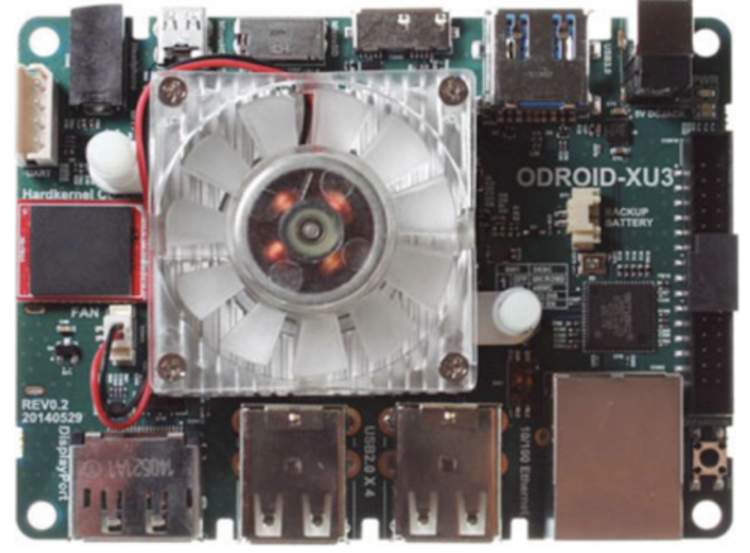
\includegraphics[width=0.7 \textwidth]{img/cap2/OdroidXU3-ES}
\caption{Odroid XU3 ES - designed to space exploration \cite{marwedel2018}}
\label{fig:OdroidXU3-ES}
\end{center}
\end{figure}



These features is strongly necessary in the AT area. For example, an important requirement is to allow for different protocols to establish communication between embedded devices and computers, such as wireless, Ethernet and Internet.

Nowadays, there exist many different kinds of Microcontrollers. Each has it own specific hardware definition, libraries and models, for example, Arduino CC\footnote{Arduino website: https://www.arduino.cc/} and Microchip\footnote{Microchip website: http://www.microchip.com/}.

\section{Final remarks}

This chapter covers essential concepts to this thesis development. It takes into account the necessary adaptations to the users' limitations, when dealing with the PW control interfaces and also the lack of resources/difficulties to travel to the training centers. Presented technological subjects (software/hardware)  helps to trigger the PW remotely and also, to collect and transmit control signals. In addition, it also discusses how to develop a safe and adaptative training environment using AR or VR techniques. Moreover, it has been pointed up the relevance to evaluate the user's performance during the sessions. These fundamentals give support to understand how to develop, integrate, and share the resources to be accessed by users from anywhere by needing only Internet access.

Next chapter presents related work considering Telerehabilitation applications and systems supported by VR and AR technology for the training of PW